\documentclass[12pt]{article}

%%%%%%%%%%%%%%%%%%%%%%%%%%%%%%%%%%%%%%%%%%%%%%%%%%%%%%%%%%%%%%%%%%%%%%%%%%%%%%%%
%                           Package preset for homework
%%%%%%%%%%%%%%%%%%%%%%%%%%%%%%%%%%%%%%%%%%%%%%%%%%%%%%%%%%%%%%%%%%%%%%%%%%%%%%%%
% Miscellaneous
\usepackage[margin=1in]{geometry}
\usepackage[utf8]{inputenc}
\usepackage{indentfirst}
\usepackage{blindtext}
\usepackage{graphicx}
\usepackage{xr-hyper}
\usepackage{hyperref}
\usepackage{enumitem}
\usepackage{color}
\usepackage{float}
% Math
\usepackage{latexsym}
\usepackage{amsfonts}
\usepackage{amssymb}
\usepackage{amsmath}
\usepackage{commath}
\usepackage{amsthm}
\usepackage{bbold}
\usepackage{bm}
% Physics
\usepackage{physics}
\usepackage{siunitx}
% Code typesetting
\usepackage{listings}
% Citation
\usepackage[authoryear]{natbib}
\usepackage{appendix}
\usepackage[capitalize]{cleveref}
% Title & name
\title{Homework}
\author{Tien Vo}
\date{\today}


%%%%%%%%%%%%%%%%%%%%%%%%%%%%%%%%%%%%%%%%%%%%%%%%%%%%%%%%%%%%%%%%%%%%%%%%%%%%%%%%
%                   User-defined commands and environments
%%%%%%%%%%%%%%%%%%%%%%%%%%%%%%%%%%%%%%%%%%%%%%%%%%%%%%%%%%%%%%%%%%%%%%%%%%%%%%%%
%%% Misc
\sisetup{load-configurations=abbreviations}
\newcommand{\due}[1]{\date{Due: #1}}
\newcommand{\hint}{\textit{Hint}}
\let\oldt\t
\renewcommand{\t}[1]{\text{#1}}

%%% Bold sets & abbrv
\newcommand{\N}{\mathbb{N}}
\newcommand{\Z}{\mathbb{Z}}
\newcommand{\R}{\mathbb{R}}
\newcommand{\Q}{\mathbb{Q}}
\let\oldP\P
\renewcommand{\P}{\mathbb{P}}
\newcommand{\LL}{\mathcal{L}}
\newcommand{\FF}{\mathcal{F}}
\newcommand{\HH}{\mathcal{H}}
\newcommand{\NN}{\mathcal{N}}
\newcommand{\ZZ}{\mathcal{Z}}
\newcommand{\RN}[1]{\textup{\uppercase\expandafter{\romannumeral#1}}}
\newcommand{\ua}{\uparrow}
\newcommand{\da}{\downarrow}

%%% Unit vectors
\newcommand{\xhat}{\vb{\hat{x}}}
\newcommand{\yhat}{\vb{\hat{y}}}
\newcommand{\zhat}{\vb{\hat{z}}}
\newcommand{\nhat}{\vb{\hat{n}}}
\newcommand{\rhat}{\vb{\hat{r}}}
\newcommand{\phihat}{\bm{\hat{\phi}}}
\newcommand{\thetahat}{\bm{\hat{\theta}}}

%%% Other math stuff
\providecommand{\units}[1]{\,\ensuremath{\mathrm{#1}}\xspace}
% Set new style for problem
\newtheoremstyle{problemstyle}  % <name>
        {10pt}                   % <space above>
        {10pt}                   % <space below>
        {\normalfont}           % <body font>
        {}                      % <indent amount}
        {\bfseries\itshape}     % <theorem head font>
        {\normalfont\bfseries:} % <punctuation after theorem head>
        {.5em}                  % <space after theorem head>
        {}                      % <theorem head spec (can be left empty, 
                                % meaning `normal')>

% Set problem environment
\theoremstyle{problemstyle}
\newtheorem{problemenv}{Problem}[section]
\newenvironment{problem}[1]{%
  \renewcommand\theproblemenv{#1}%
  \problemenv
}{\endproblemenv}
% Set lemma environment
\newenvironment{lemma}[2][Lemma]{\begin{trivlist}
\item[\hskip \labelsep {\bfseries #1}\hskip \labelsep {\bfseries #2.}]}{\end{trivlist}}
% Set solution environment
\newenvironment{solution}{
    \begin{proof}[Solution]$ $\par\nobreak\ignorespaces
}{\end{proof}}
\numberwithin{equation}{problemenv}

%%% Page format
\setlength{\parindent}{0.5cm}
\setlength{\oddsidemargin}{0in}
\setlength{\textwidth}{6.5in}
\setlength{\textheight}{8.8in}
\setlength{\topmargin}{0in}
\setlength{\headheight}{18pt}

%%% Code environments
\definecolor{dkgreen}{rgb}{0,0.6,0}
\definecolor{gray}{rgb}{0.5,0.5,0.5}
\definecolor{mauve}{rgb}{0.58,0,0.82}
\lstset{frame=tb,
  language=Python,
  aboveskip=3mm,
  belowskip=3mm,
  showstringspaces=false,
  columns=flexible,
  basicstyle={\small\ttfamily},
  numbers=none,
  numberstyle=\tiny\color{gray},
  keywordstyle=\color{blue},
  commentstyle=\color{dkgreen},
  stringstyle=\color{mauve},
  breaklines=true,
  breakatwhitespace=true,
  tabsize=4
}
\lstset{
  language=Mathematica,
  numbers=left,
  numberstyle=\tiny\color{gray},
  numbersep=5pt,
  breaklines=true,
  captionpos={t},
  frame={lines},
  rulecolor=\color{black},
  framerule=0.5pt,
  columns=flexible,
  tabsize=2
}


\title{Homework 13: Phys 7310 (Fall 2021)}

\begin{document}
\maketitle
%%%%%%%%%%%%%%%%%%%%%%%%%%%%%%%%%%%%%%%%%%%%%%%%%%%%%%%%%%%%%%%%%%%%%%%%%%%%%%%
\begin{problem}{13.1}[A wave packet]
An approximately monochromatic plane wave packet in one dimension has the
instantaneous form, $u(x,0)=f(x)e^{ik_0x}$, with $f(x)=Ne^{-\alpha\abs{x}/2}$
the modulation envelope. Calculate the wave-number spectrum $\abs{A(k)}^2$ of
the packet, sketch $\abs{u(x,0)}^2$ and $\abs{A(k)}^2$, evaluate explicitly the
rms deviations from the means $\Delta x$ and $\Delta k$ (defined in terms of the
intensity $\abs{u(x,0)}^2$ and $\abs{A(k)}^2$), and test inequality (7.82).
\begin{solution}
By definition,
\begin{align}
    A(k)
    &=\frac1{\sqrt{2\pi}}\int_{-\infty}^\infty dx
    e^{-ikx}\qty[u(x,0)+\frac{i}{\omega}\frac{\partial u}{\partial
    t}(x,0)]\notag\\
    &=\frac{N}{\sqrt{2\pi}}\int_{-\infty}^\infty
    dxe^{-ikx}e^{-\alpha\abs{x}/2}e^{ik_0x}\notag\\
    &=\frac{N}{\sqrt{2\pi}}\qty[\int_{-\infty}^0dxe^{i(k_0-k)x}e^{\alpha
    x/2}+\int_0^\infty dxe^{i(k_0-k)x}e^{-\alpha x/2}]\notag\\
    &=\frac{N}{\sqrt{2\pi}}\qty[\frac{2i}{2(k-k_0)+i\alpha}+\frac{2}{2i(k-k_0)+\alpha}]\notag\\
    &=\frac{N}{\sqrt{2\pi}}\frac{4\alpha}{4(k-k_0)^2+\alpha^2}
\end{align}
Then it follows that
\begin{align}
    \abs{A(k)}^2=\frac8\pi\frac{N^2\alpha^2}{[4(k-k_0)^2+\alpha^2]^2} 
\end{align}
For $N=\alpha=k_0=1$, we plot $\abs{u}^2$ and $\abs{A}^2$ as follows
\begin{center}
    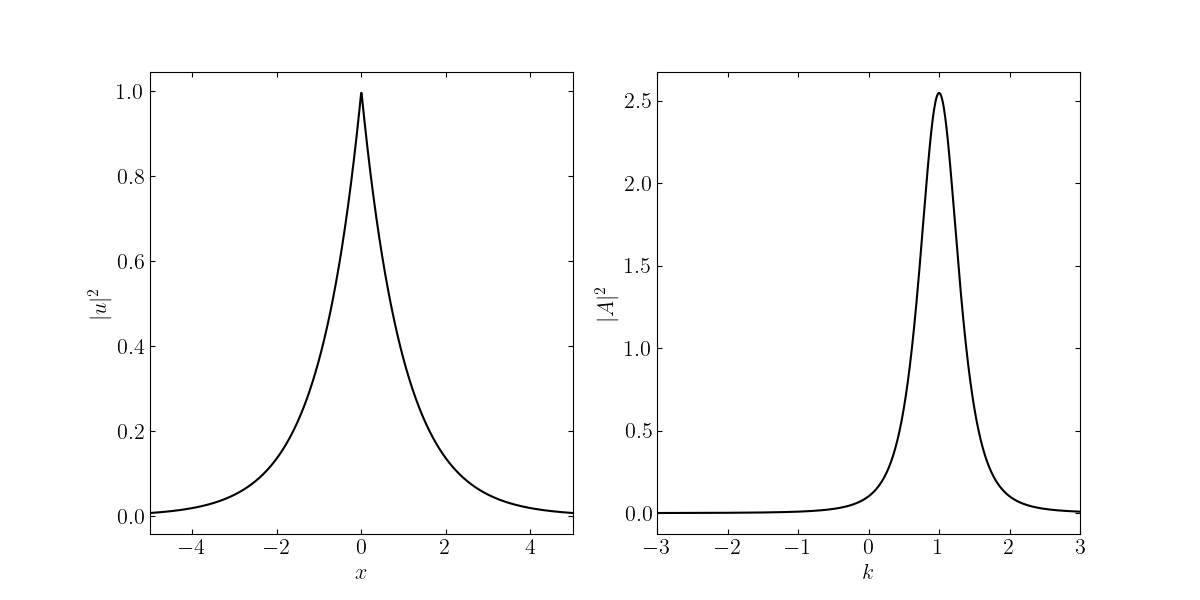
\includegraphics[width=0.9\textwidth]{p1.png} 
\end{center}

For $\Delta x$, the kernel is already symmetric about $x=0$. So by definition,
\begin{equation}
    \abs{x^2}=N^2\int_{-\infty}^\infty dx x^2e^{-\alpha\abs{x}}
    =N^2\qty[\int_{-\infty}^0 dxx^2e^{\alpha x}+\int_0^\infty dxx^2e^{-\alpha
    x}]=\frac{4N^2}{\alpha^3}
\end{equation}
Similarly, we calculate
\begin{equation}
    \mathcal{N}_x=\int_{-\infty}^\infty dx\abs{u(x,0)}^2
    =\int_{-\infty}^0dx e^{\alpha x}+\int_0^\infty dxe^{-\alpha x}
    =\frac{2N^2}{\alpha} 
\end{equation}
Then it follows that $\Delta x=\sqrt{\abs{x^2}/\mathcal{N}_x}=\sqrt2/\alpha$.
Now, since the kernel for $k$ ($\abs{A}^2$) is not symmetric, we can shift it by
$k\mapsto k+k_0$ such that
\begin{equation}
    \abs{A(k)}^2=\frac8\pi\frac{N^2\alpha^2}{(4k^2+\alpha^2)^2} 
\end{equation}
Then
\begin{align}
    \mathcal{N}_k=\frac{8N^2\alpha^2}{\pi}\int_{-\infty}^\infty\frac{dk}{(4k^2+\alpha^2)^2}=\frac{2N^2}{\alpha} 
\end{align}
and
\begin{align}
    \expval{k^2}
    =\frac{8N^2\alpha^2}{\pi}\int_{-\infty}^\infty\frac{k^2dk}{(4k^2+\alpha^2)^2}
    =\frac{N^2\alpha}{2}
\end{align}
Thus, $\Delta k=\sqrt{\expval{k^2}/\mathcal{N}_k}=\alpha/2$. Then
\begin{equation}
    \Delta x\Delta k=\frac1{\sqrt2}\approx0.71>\frac12 
\end{equation}
So the inequality (7.82) is satisfied.
\end{solution}
\end{problem}
%%%%%%%%%%%%%%%%%%%%%%%%%%%%%%%%%%%%%%%%%%%%%%%%%%%%%%%%%%%%%%%%%%%%%%%%%%%%%%%    
%%%%%%%%%%%%%%%%%%%%%%%%%%%%%%%%%%%%%%%%%%%%%%%%%%%%%%%%%%%%%%%%%%%%%%%%%%%%%%%
\begin{problem}{13.2}[A triangular waveguide]
A waveguide is constructed so that the cross section of the guide forms a right
triangle with side of length $a$, $a$, $\sqrt2a$, as shown. The medium inside
has $\mu_r=\epsilon_r=1$. Assuming infinite conductivity for the walls,
determine the possible modes of propagation and their cutoff frequencies.
\begin{solution}
First, the TE solution for a square waveguide from (8.42, Jackson) is
\begin{equation}\label{p2:psi_TE}
    \psi=H_0\cos\qty(\frac{m\pi x}{a})\cos\qty(\frac{n\pi y}{a}) 
\end{equation}
which already satisfies the boundary conditions that $\partial\psi/\partial n=0$
at $y=0$ and $x=a$. Now, if the diagonal of the triangular waveguide is defined
by the line $y=x$, then it must follow also that
\begin{equation}
    \eval{\frac{\partial\psi}{\partial n}}_{y=x}
    =\eval{\frac1{\sqrt2}(-\xhat+\yhat)\vdot\grad\psi}_{y=x}
    =\eval{\frac1{\sqrt{2}}\qty(\frac{\partial\psi}{\partial
    y}-\frac{\partial\psi}{\partial x})}_{y=x}=0
\end{equation}
or equivalently, that
\begin{equation}
    \eval{\frac{\partial\psi}{\partial x}}_{y=x}
    =\eval{\frac{\partial\psi}{\partial y}}_{y=x} 
\end{equation}
This means the function $\psi$ has to be symmetric under the
transformation $x\mapsto y$ and $y\mapsto x$. However, \eqref{p2:psi_TE} is not
symmetric. But we can rewrite $\psi$ as a linear combination
\begin{equation}\label{p2:tri_TE}
    \psi=\frac{H_0}{\sqrt{2}}\qty[\cos\qty(\frac{m\pi
    x}{a})\cos\qty(\frac{n\pi y}{a})+\cos\qty(\frac{n\pi
x}{a})\cos\qty(\frac{m\pi y}{a})] 
\end{equation}
so that
\begin{align}
    \eval{\qty(\frac{\partial\psi}{\partial y}-\frac{\partial\psi}{\partial
    x})}_{y=x}
    &\sim-\frac{n\pi}{a}\cos\qty(\frac{m\pi x}{a})\sin\qty(\frac{n\pi y}{a})
    -\frac{m\pi}{a}\cos\qty(\frac{n\pi x}{a})\sin\qty(\frac{m\pi y}{a})\notag\\
    &\qquad+\frac{m\pi}{a}\sin\qty(\frac{m\pi x}{a})\cos\qty(\frac{n\pi}{a})
    +\frac{n\pi}{a}\sin\qty(\frac{n\pi x}{a})\cos\qty(\frac{m\pi y}{a})\notag\\
    &=0
\end{align}
where the last equality is true only at $y=x$. Thus, the TE solution for the
triangular waveguide is \eqref{p2:tri_TE}. Then from (8.34, Jackson), we can
find
\begin{align}
    \laplacian_t\psi
    =\frac{\partial^2\psi}{\partial x^2}+\frac{\partial^2\psi}{\partial
    y^2}
    =-\qty(\frac{m^2\pi^2}{a^2}+\frac{n^2\pi^2}{a^2})\psi
    =-\gamma_{mn}^2\psi
\end{align}
Thus, $\gamma_{mn}=(\pi/a)\sqrt{m^2+n^2}$. The allowed modes are $m,n\geq0$, but
$m$ and $n$ cannot be both zero because $\psi$ is then not periodic. The cutoff
frequency is thus defined by $(m=0,n=1)$ or $(m=1,n=0)$
\begin{equation}
    \omega_{TE}=\frac{\gamma_{10}}{\sqrt{\mu_0\epsilon_0}}
    =\frac{\gamma_{01}}{\sqrt{\mu_0\epsilon_0}}
    =\frac{c\pi}{a}
\end{equation}

Now, regarding the TM solution for the square waveguide, $\psi=E_z$ has to
vanish at $x=0,a$ and $y=0,a$. So instead of cosine function, $\psi$ is
\begin{equation}
    \psi=E_0\sin\qty(\frac{m\pi x}{a})\sin\qty(\frac{n\pi y}{a}) 
\end{equation}
Now, at the diagonal $y=x$, it must follow also that
\begin{equation}
    \eval{\psi}_{y=x}=0 
\end{equation}
This condition requires that $\psi$ must be antisymmetric, instead. But $\psi$
as is, is not antisymmetric. So we can rewrite $\psi$ as a linear combination
\begin{equation}\label{p2:tri_TM}
    \psi=\frac{E_0}{\sqrt2}\qty[\sin\qty(\frac{m\pi
    x}{a})\sin\qty(\frac{n\pi y}{a})-\sin\qty(\frac{n\pi
x}{a})\sin\qty(\frac{m\pi y}{a})] 
\end{equation}
so that at $y=x$, 
\begin{equation}
    \psi\sim\sin\qty(\frac{m\pi x}{a})\sin\qty(\frac{n\pi x}{a})
    -\sin\qty(\frac{n\pi x}{a})\sin\qty(\frac{m\pi x}{a})
    =0
\end{equation}
Thus, \eqref{p2:tri_TM} is the TM solution for the triangular waveguide. Similar
to the TE case, from (8.34, Jackson),
\begin{equation}
    \laplacian_t\psi=-\frac{\pi^2}{a^2}(m^2+n^2)\psi=-\gamma_{mn}^2\psi
\end{equation}
Thus, $\gamma_{mn}$ is still the same as the TE case. However, $m,n$ are not
allowed to be zero because that leads to a trivial solution. Also, $m\neq n$
because that also leads to a trivial solution due to the antisymmetry of the
function if $m=n$. The ground case is then $(m=1,n=2)$ or $(m=2,n=1)$, in which 
the cutoff frequency is
\begin{equation}
    \omega_{TM}=\frac{\gamma_{12}}{\sqrt{\mu_0\epsilon_0}}=\frac{\gamma_{21}}{\sqrt{\mu_0\epsilon_0}}=\frac{c\pi}{a}\sqrt{5} 
\end{equation}
\end{solution}
\end{problem}
%%%%%%%%%%%%%%%%%%%%%%%%%%%%%%%%%%%%%%%%%%%%%%%%%%%%%%%%%%%%%%%%%%%%%%%%%%%%%%%%
\end{document}
